\problemname{Astronoom}
\illustration{.3}{img/TychoBrahe.JPG}{}

\noindent
Astronoomil on kirg tähtede vaatamise vastu.
Erilise naudingu osaks saab ta siis, kui näeb läbi oma teleskoobi samaaegselt $k$~tähte.
Raadiusega~$r$ teleskoobi ehitamine maksab $t\cdot r$~krooni.
Vastvalminud teleskoop on esialgu suunatud punkti $(0,0)$.
Ka teleskoobi mujale suunamine võtab vaeva:
teleskoobi suuna muutmine $d$~ühiku võrra maksab $s\cdot d$~krooni.
Astronoom näeb läbi teleskoobi kõiki tähti, mis on kaugusel ülimalt $r$ punktist, kuhu
teleskoop suunatud on.

Kui palju maksab teleskoobi ehitamine ja suuna muutmine nii, et sellega oleks võimalik
$k$~tähte samaaegselt näha.

\medskip

Kõik koordinaadid ja kaugused on antud Eukleidilisel tasandil.


\section*{Näide}

Vaatleme näidet, kus on $n=3$ tähte, positsioonidel $(0,0)$, $(2,0)$ ja $(3,1)$.
Varjutatud ala kujutab teleskoopi raadiusega~$1$ suunatud punkti $(1,0)$; see katab
kaks tähte, maksab $s + t$ krooni ja on näite~$3$ optimaalne lahend.
Joonisel on kujutatud ka näidete~$1$, $2$ ja $4$ optimaalsed lahendid.

\medskip
\noindent
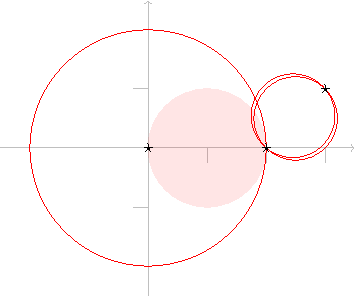
\includegraphics[width=.3\textwidth]{img/samples.pdf}


\section*{Sisend}

Sisendi esimene rida koosneb neljast täisarvust:
tähtede arv~$k$, mida astronoom soovib vaadelda;
tähtede arv~$n$ taevas;
teleskoobi ümbersuunamise hind~$s$ ja
teleskoobi ehitamise hind~$t$.
Järgnevad $n$ rida, millest $i$-ndal on $i$-nda tähe
täisarvulised koordinaadid $x_i$ ja $y_i$.

\section*{Väljund}

Üksainus reaalarv: minimaalne astronoomi poolt kulutatud rahasumma.

\section*{Piirangud ja hindamine}

Võib eeldada, et:
\begin{enumerate}
\item $1\leq k\leq n\leq 700$. % constraint:kn
\item $x_i, y_i\in \{-10^9,\ldots, 10^9\}$ iga $i\in\{1,\ldots,n\}$ kohta. % constraint:xy
\item $s,t\in \{0,\ldots, 10^9\}$. % constraint:st
\item Sinu vastus loetakse korrektseks, kui tema absoluutne või suhteline viga jääb
$\epsilon = 10^{-6}$ piiresse.
\end{enumerate}


Selles ülesandes on testid jagatud gruppidesse, iga grupp on väärt mingi arvu punkte.
Iga grupi eest saavad punkte vaid need lahendused, mis läbivad kõik sellesse gruppi kuuluvad testid.
Sinu lõplik skoor on esituste maksimum.

\medskip
\noindent
\begin{tabular}{lll}
  Grupp & Punktid & Lisapiirangud\\\hline
  $1$ & $18$ &  $t\leq s$\\
  $2$ & $17$ & $n\le 50$ ja $s=0$\\
  $3$ & $15$ & $s=0$\\
  $4$ & $12$ & $n\leq 50$\\
  $5$ & $14$ & $n\leq 350$\\
  $6$ & $10$ & $\epsilon = 1/10$\\
  $7$ & $14$ & \emph{Lisapiirangud puuduvad}\\
\end{tabular}
